\begin{tikzpicture}
  \node[inner sep=0] (torusfield) {%
    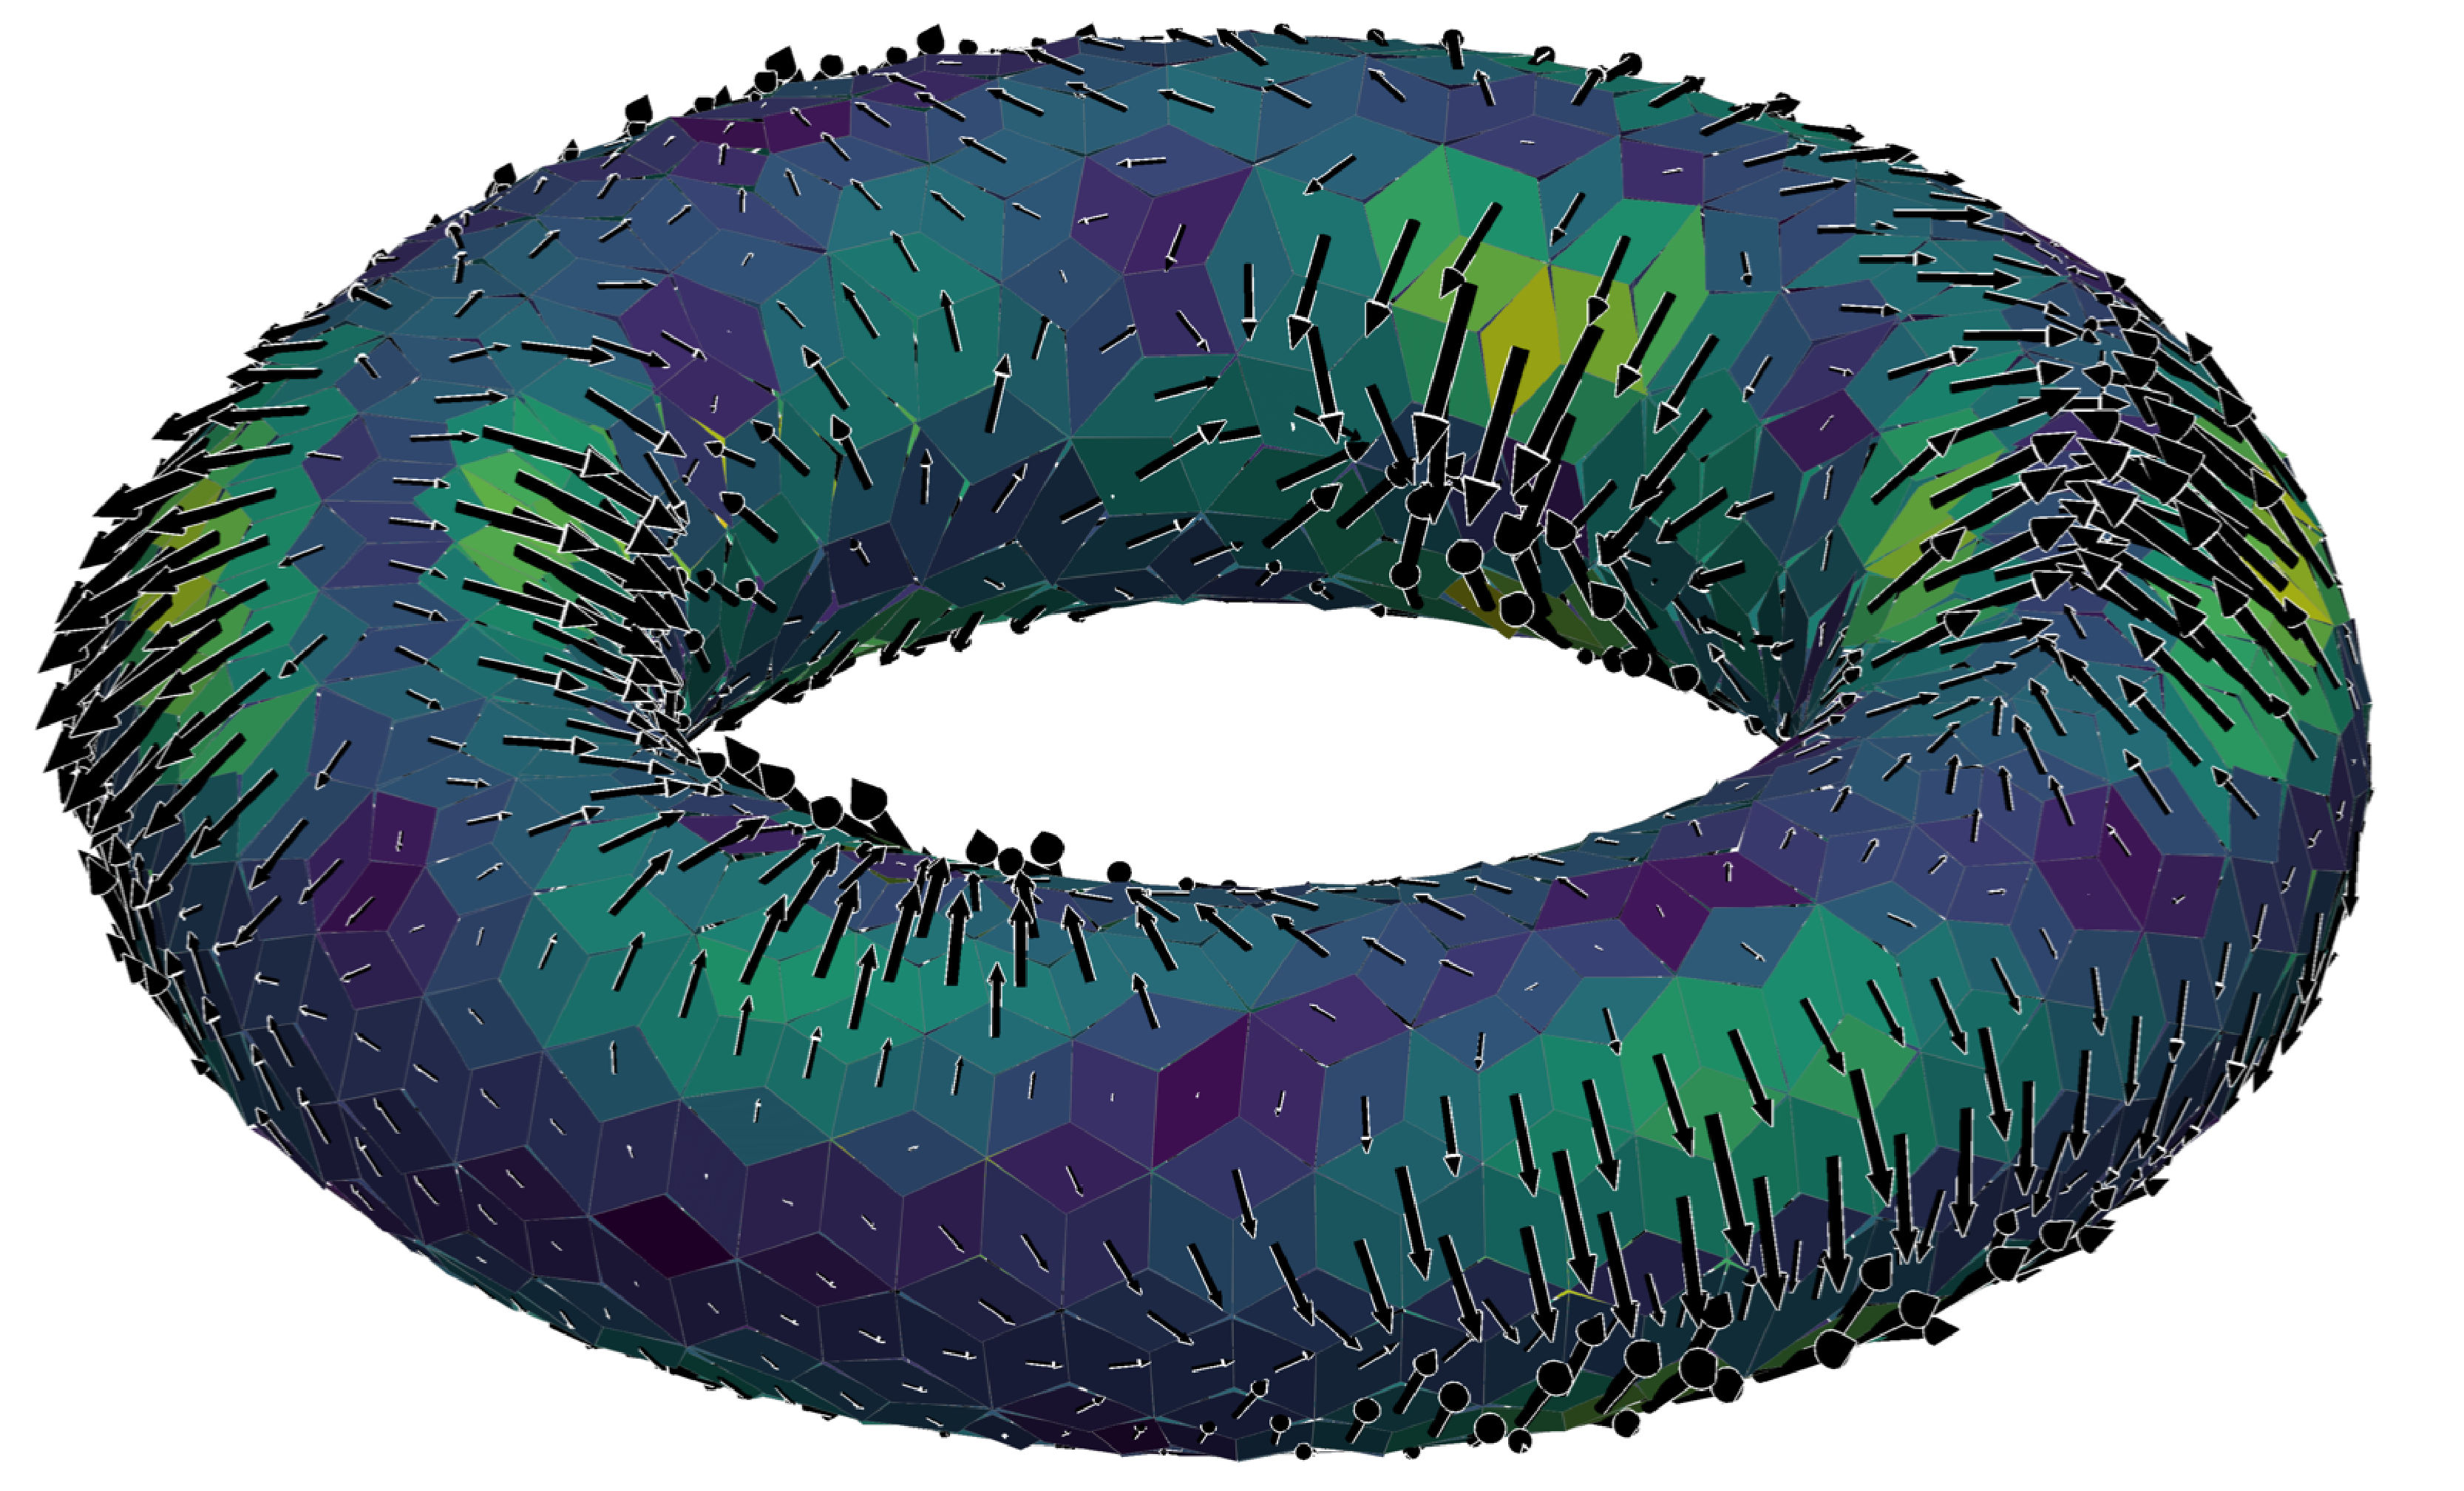
\includegraphics[width=0.7\textwidth]{img/torus_ddfv_gradient.pdf}%
  };

\iffalse
  \path let \p1=(torusfield.south west), \p2=(torusfield.north west) in
    \pgfextra{\xdef\torusfieldheight{\the\dimexpr\y2-\y1\relax}};
  \pgfplotscolorbardrawstandalone[
    colormap name=viridis,
    point meta min=3.228900e-03,
    point meta max=1.853583e+00,
    parent axis height=\torusfieldheight,
    colorbar style={
      at={(torusfield.east)},
      anchor=east,
      height=0.5*\torusfieldheight,
      width=5pt,
      ytick={1},
      yticklabels={$1$},
      ylabel={$\norme{\grad^\ensdiamantplat u^\ensddfvplat - \grad_\surflisse \, u}_2$},
      ylabel style={rotate=-90},
    },
  ]
\fi
\end{tikzpicture}
